% Bootstrap Capability: Prompt-Managed Workflow Engineering
% A White Paper on Iterative Spec-Driven Development
\documentclass[11pt,letterpaper]{article}

% Packages
\usepackage[utf8]{inputenc}
\usepackage[margin=1in]{geometry}
\usepackage{amsmath,amssymb}
\usepackage{listings}
\usepackage{xcolor}
\usepackage{hyperref}
\usepackage{booktabs}
\usepackage{graphicx}
\usepackage{tikz}
\usepackage{fancyhdr}
\usepackage{tcolorbox}

\usetikzlibrary{shapes.geometric, arrows.meta, positioning, fit, backgrounds}

% Hyperref setup
\hypersetup{
    colorlinks=true,
    linkcolor=blue,
    citecolor=blue,
    urlcolor=blue,
    pdftitle={Bootstrap Capability: Prompt-Managed Workflow Engineering},
    pdfauthor={NOAA EMC Global Workflow MCP Team}
}

% Code listing setup
\lstset{
    basicstyle=\ttfamily\footnotesize,
    breaklines=true,
    frame=single,
    captionpos=b,
    numbers=left,
    numberstyle=\tiny\color{gray},
    keywordstyle=\color{blue},
    commentstyle=\color{green!60!black},
    stringstyle=\color{red},
    backgroundcolor=\color{gray!5}
}

% Header/Footer
\setlength{\headheight}{14pt}
\pagestyle{fancy}
\fancyhf{}
\rhead{Bootstrap Capability White Paper}
\lhead{NOAA EMC Global Workflow Team}
\cfoot{\thepage}

% Custom box for key insights
\newtcolorbox{keyinsight}{
    colback=blue!5,
    colframe=blue!75!black,
    fonttitle=\bfseries,
    title=Key Insight
}

% Title information
\title{\textbf{Bootstrap Capability:} \\
       \textbf{Prompt-Managed Workflow Engineering} \\[0.5em]
       \large A White Paper on Iterative Spec-Driven Development}

\author{
    NOAA EMC Global Workflow MCP Team \\
    Environmental Modeling Center \\
    National Oceanic and Atmospheric Administration \\
    \texttt{Terry.McGuinness@noaa.gov}
}

\date{January 6, 2026}

\begin{document}

\maketitle

\begin{abstract}
We present \textbf{Bootstrap Capability}, an extension to the Spec-Driven Development (SDD) framework that enables AI-assisted workflow engineering through iterative prompt-managed specification development. The system introduces a two-phase execution model: \texttt{dry\_run} for plan validation and \texttt{supervised} for controlled execution with human approval gates. This approach bridges the gap between natural language task descriptions and executable workflow specifications, enabling a rapid development cycle where AI drafts specifications, humans validate through dry-run preview, and execution proceeds with oversight. We demonstrate this capability through implementation in the MCP/RAG system for NOAA Global Workflow, achieving autonomous code generation with full auditability and rollback support.

\textbf{Keywords:} Spec-Driven Development, Bootstrap Capability, Workflow Engineering, AI-Assisted Development, Model Context Protocol
\end{abstract}

%------------------------------------------------------------------------------
\section{Introduction}
%------------------------------------------------------------------------------

Modern software development increasingly relies on AI assistance for code generation, documentation, and system maintenance. However, a fundamental challenge remains: how do we ensure AI-generated actions align with human intent while maintaining the efficiency gains of automation?

The \textbf{Bootstrap Capability} addresses this challenge by introducing a structured workflow engineering process where:

\begin{enumerate}
    \item Specifications are written in human-readable Markdown
    \item AI assistants can draft these specifications through prompt engineering
    \item A \texttt{dry\_run} mode validates specifications without execution
    \item A \texttt{supervised} mode executes with human approval at each side-effect step
\end{enumerate}

This paper describes the conceptual foundation, execution model, and practical implementation of this capability within the SDD framework.

%------------------------------------------------------------------------------
\section{The Iterative Development Loop}
%------------------------------------------------------------------------------

The Bootstrap Capability establishes a feedback loop between prompt engineering (AI-assisted) and system execution, as illustrated in Figure~\ref{fig:dev-loop}.

\begin{figure}[h]
\centering
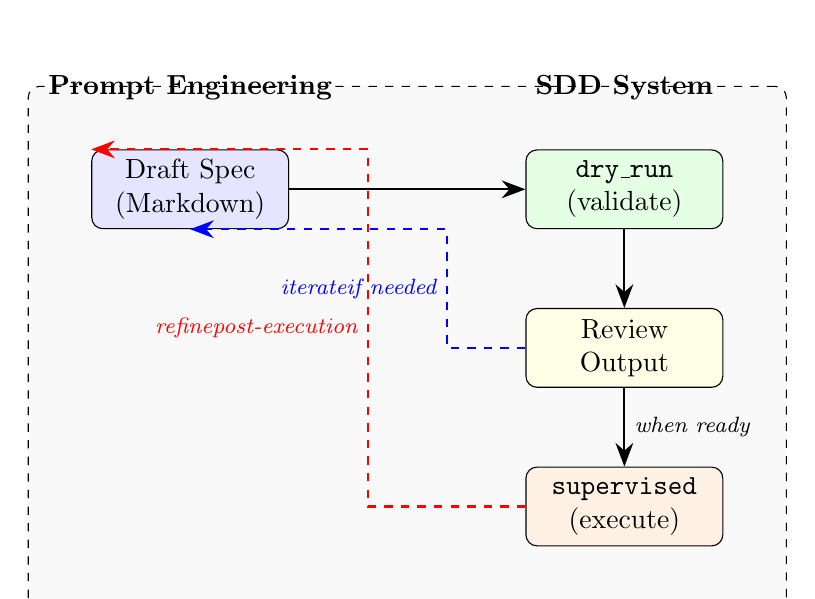
\begin{tikzpicture}[
    node distance=1.5cm,
    box/.style={rectangle, draw, rounded corners, minimum width=2.5cm, minimum height=1cm, align=center, fill=white},
    arrow/.style={-{Stealth[length=3mm]}, thick},
    label/.style={font=\footnotesize\itshape}
]

% Left side - Prompt Engineering
\node[box, fill=blue!10] (draft) {Draft Spec\\(Markdown)};

% Right side - SDD System
\node[box, fill=green!10, right=3cm of draft] (dryrun) {\texttt{dry\_run}\\(validate)};
\node[box, fill=yellow!10, below=1cm of dryrun] (review) {Review\\Output};
\node[box, fill=orange!10, below=1cm of review] (supervised) {\texttt{supervised}\\(execute)};

% Arrows
\draw[arrow] (draft) -- (dryrun);
\draw[arrow] (dryrun) -- (review);
\draw[arrow] (review) -- node[right, label] {when ready} (supervised);

% Feedback loops
\draw[arrow, dashed, blue] (review.west) -- ++(-1,0) |- node[left, pos=0.25, label] {iterate\\if needed} (draft.south);
\draw[arrow, dashed, red] (supervised.west) -- ++(-2,0) |- node[left, pos=0.25, label] {refine\\post-execution} (draft.north west);

% Labels for sections
\node[above=0.5cm of draft, font=\bfseries] {Prompt Engineering};
\node[above=0.5cm of dryrun, font=\bfseries] {SDD System};

% Surrounding box
\begin{scope}[on background layer]
    \node[draw, dashed, rounded corners, fit=(draft)(dryrun)(review)(supervised), inner sep=0.8cm, fill=gray!5] {};
\end{scope}

\end{tikzpicture}
\caption{The Iterative Development Loop: AI-assisted specification drafting feeds into the SDD system's validation and execution phases, with feedback loops for refinement.}
\label{fig:dev-loop}
\end{figure}

\subsection{Phase Descriptions}

\begin{description}
    \item[Draft Spec] An AI assistant (Claude, Copilot, etc.) or human author creates a workflow specification in Markdown format. The specification defines steps, types, targets, and validation criteria.
    
    \item[\texttt{dry\_run}] The system parses the specification and reports what actions \textit{would} occur without executing anything. This is analogous to \texttt{terraform plan} or Claude CLI's \texttt{/plan} mode.
    
    \item[Review Output] The human reviews the dry-run output to verify the plan matches intent. If issues are found, the specification is refined and re-validated.
    
    \item[\texttt{supervised}] Once satisfied with the plan, the human triggers supervised execution. The system executes each step, pausing for approval before any side-effect operation (file creation, command execution, database modification).
\end{description}

%------------------------------------------------------------------------------
\section{Execution Modes}
%------------------------------------------------------------------------------

The Bootstrap Capability distinguishes between two fundamental execution modes, summarized in Table~\ref{tab:modes}.

\begin{table}[h]
\centering
\caption{Comparison of Execution Modes}
\label{tab:modes}
\begin{tabular}{@{}lcccc@{}}
\toprule
\textbf{Mode} & \textbf{Creates Code} & \textbf{Runs Commands} & \textbf{Approval Gates} & \textbf{Changes Persist} \\
\midrule
\texttt{dry\_run}   & No  & No  & No  & N/A \\
\texttt{supervised} & Yes & Yes & Yes & Yes \\
\bottomrule
\end{tabular}
\end{table}

\begin{keyinsight}
\texttt{dry\_run} is \textbf{not} sandboxed execution---it is pure specification parsing. No code runs, no files are created, no side effects occur. It answers: ``What does this workflow \textit{intend} to do?''

\texttt{supervised} is \textbf{real execution} with human oversight. When you approve a step, the action occurs on the live system. It answers: ``May I proceed with this action?''
\end{keyinsight}

\subsection{Side-Effect Classification}

The system classifies workflow steps into two categories:

\begin{itemize}
    \item \textbf{Read-only steps} (auto-execute): \texttt{health\_check}, \texttt{validation}, \texttt{data\_query}, \texttt{analysis}
    \item \textbf{Side-effect steps} (require approval): \texttt{code\_generation}, \texttt{code\_modification}, \texttt{command}, \texttt{ingestion}, \texttt{file\_delete}, \texttt{git\_operation}
\end{itemize}

In supervised mode, read-only steps execute automatically while side-effect steps pause for human approval.

%------------------------------------------------------------------------------
\section{Workflow Specification Format}
%------------------------------------------------------------------------------

Workflows are defined in Markdown with structured metadata. A well-formed step specification includes:

\begin{lstlisting}[caption={Example Workflow Step Specification}]
### Step 3: Generate Example Tool
**Type**: code_generation
**Target**: mcp_server_node/src/tools/ExampleTool.js
**Template**: basic-mcp-tool
**Required**: Yes
**Variables**:
- className: ExampleTool
- toolName: example_operation

Generate a new MCP tool using the template system.
\end{lstlisting}

The parser extracts:
\begin{itemize}
    \item Step name and number (from heading)
    \item Type (determines execution handler)
    \item Target (file path, command, etc.)
    \item Template (for code generation)
    \item Variables (interpolated into templates)
    \item Required flag (fail workflow if step fails)
\end{itemize}

%------------------------------------------------------------------------------
\section{Implementation: Bootstrap Capability Demo}
%------------------------------------------------------------------------------

We demonstrate the Bootstrap Capability through a workflow that generates a functional MCP tool:

\begin{enumerate}
    \item \textbf{Health Check}: Verify system components are operational
    \item \textbf{Validate Knowledge Base}: Confirm RAG system is healthy
    \item \textbf{Generate Code}: Create \texttt{ExampleBootstrapTool.js} from template
    \item \textbf{Validate File Exists}: Confirm file was created
    \item \textbf{Validate Syntax}: Run \texttt{node --check} on generated file
    \item \textbf{Validate Content}: Verify class definition exists in file
    \item \textbf{Cleanup} (optional): Remove generated file after demo
\end{enumerate}

\subsection{Template System}

Code generation uses interpolated templates stored in \texttt{src/templates/}:

\begin{lstlisting}[caption={Template Variable Interpolation}]
/**
 * {{className}} - {{description}}
 * Generated by SDD Bootstrap Capability
 * Date: {{generatedDate}}
 */
export class {{className}} {
  registerWith(server) {
    server.tool('{{toolName}}', '{{toolDescription}}', ...);
  }
}
\end{lstlisting}

\subsection{Transaction Management}

All modifications occur within a transaction that supports rollback:

\begin{lstlisting}[caption={Transaction Flow}]
BEGIN TRANSACTION 'bootstrap_capability_demo'
  |-- Create backup directory
  |-- Execute Step 3 (code_generation)
  |      +-- Track: file created, path stored
  |-- Execute Step 4-6 (validation)
  |      +-- If ANY fails -> ROLLBACK
  +-- Cleanup (optional)
COMMIT TRANSACTION (or ROLLBACK on failure)
\end{lstlisting}

%------------------------------------------------------------------------------
\section{Comparison with Related Approaches}
%------------------------------------------------------------------------------

\begin{table}[h]
\centering
\caption{Comparison with Related Development Approaches}
\label{tab:comparison}
\begin{tabular}{@{}lccc@{}}
\toprule
\textbf{Approach} & \textbf{Spec Format} & \textbf{Preview Mode} & \textbf{Approval Gates} \\
\midrule
Traditional Coding    & N/A (code is spec) & No  & No  \\
Terraform/IaC         & HCL/YAML           & Yes (\texttt{plan}) & No  \\
Claude CLI            & Natural Language   & Yes (\texttt{/plan}) & Limited \\
GitHub Actions        & YAML               & No (dry-run limited) & Manual triggers \\
\textbf{SDD Bootstrap} & \textbf{Markdown} & \textbf{Yes} (\texttt{dry\_run}) & \textbf{Yes} (per-step) \\
\bottomrule
\end{tabular}
\end{table}

The SDD Bootstrap approach uniquely combines human-readable specifications (Markdown) with both preview and fine-grained approval capabilities.

%------------------------------------------------------------------------------
\section{Conclusion}
%------------------------------------------------------------------------------

The Bootstrap Capability extends the SDD framework with a practical methodology for AI-assisted workflow engineering:

\begin{enumerate}
    \item \textbf{Specification as Source of Truth}: Markdown workflows define intent before execution
    \item \textbf{Iterative Refinement}: \texttt{dry\_run} enables rapid validation without side effects
    \item \textbf{Controlled Execution}: \texttt{supervised} mode provides human oversight at critical points
    \item \textbf{Auditability}: Transaction management enables rollback and change tracking
\end{enumerate}

This approach bridges the gap between AI capability and human oversight, enabling systems to ``bootstrap'' their own development while maintaining the safety guarantees required for operational software.

\subsection{Future Work}

\begin{itemize}
    \item \textbf{Sandboxed Execution}: True isolation via containers or feature branches
    \item \textbf{Multi-Agent Workflows}: USD (Unsupervised Development) for sub-agent task dispatch
    \item \textbf{Automated Spec Generation}: AI generates workflow specs from natural language requirements
    \item \textbf{Continuous Integration}: \texttt{auto\_approved} mode with manifest-based pre-approval for CI/CD
\end{itemize}

%------------------------------------------------------------------------------
% References (if needed)
%------------------------------------------------------------------------------

\section*{Acknowledgments}

This work was developed as part of the NOAA Global Workflow MCP/RAG project, supporting AI-assisted development for operational weather forecasting systems.

\end{document}
